\documentclass[11 pt,t]{beamer}
\usetheme[
	bullet=circle,		% Other option: square
	bigpagenumber,		% circled page number on lower right
	topline=true,		% colored bar at the top of the frame 
	]{Zurich}

%-----------------------------------------------------------------------------
% For Drawing Diagramms in TeX
\usepackage{tikz}
\usetikzlibrary{shapes,arrows,positioning,shadows,automata}

% Define block styles used later

\tikzstyle{model}=[draw, fill=blue!20, text width=5em, 
    text centered, minimum height=2.5em,
    rounded corners,drop shadow]
\tikzstyle{m2tengine}=[draw, fill=red!20, text width=10em, 
    text centered, minimum height=2.5em,
    rounded corners,drop shadow]
%-----------------------------------------------------------------------------
% For Including Code
\usepackage{listings}

%-----------------------------------------------------------------------------
% For Citing
\usepackage[style=authoryear-comp,backend=biber]{biblatex}
\addbibresource{references.bib}

%-----------------------------------------------------------------------------
% For putting slides in Appendix
\usepackage{appendixnumberbeamer}

\usepackage{subcaption} 
%-----------------------------------------------------------------------------
% Rotating Table Headers
\newcommand\tabrotate[1]{\rotatebox{90}{#1\hspace{\tabcolsep}}}

%-----------------------------------------------------------------------------
% DOCUMENT PROPERTIES

\author{Tim Schneider}
\title{Domain-Specific Modeling}

%-----------------------------------------------------------------------------
% Bullet points in table of content
\setbeamertemplate{section in toc}[circle]
\setbeamertemplate{subsection in toc}[circle]

    
%-----------------------------------------------------------------------------


\begin{document}


% ----------------------------------------------------------------------------
\frame{

\titlepage

}
% ----------------------------------------------------------------------------
% Das Inhaltsverzeichnis
\begin{frame}
\vspace{.5cm}
  \frametitle{Contents}
  \tableofcontents
\end{frame}

\section{Terms}
\begin{frame}
\vspace{.5cm}
  \frametitle{Important Terms}
  \begin{itemize}
    \item \textbf{Model}
      \begin{itemize}
       \item formal representation (Abstraction)
       \item certain correspondence (homomorphism)
       \item purpose (pragmatics)
      \end{itemize}
      
    \item \textbf{Domain}
      \begin{itemize}
       \item common knowledge of the requirements, concepts and functionality 
	    \\in a field of study
      \end{itemize}

    \item \textbf{Domain-Specific Modeling Languages}
    \begin{itemize}
       \item textual or graphical representation of concepts, entities and relationships
	      (only those relvant for the domain)
      \end{itemize}

  \end{itemize}
\end{frame}

\section{Motivation}
\begin{frame}

  \frametitle{Motivation}
  \begin{figure}[h]
\begin{center}
\begin{tabular}{|c|c|c|c|c|}\hline
&&&&\\
\begin{subfigure}[t]{0.15\textwidth}\centering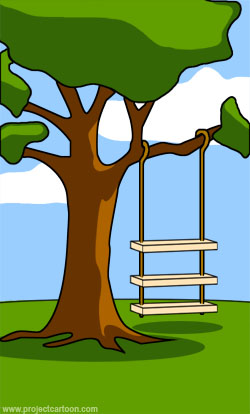
\includegraphics[width=0.9\columnwidth]{images/howexplained}
\caption*{\tiny \centering How the domain expert explained it}\label{fig:howexplained}\end{subfigure}&
\begin{subfigure}[t]{0.15\textwidth}\centering
\includegraphics[width=0.9\columnwidth]{images/howunderstood}
\caption*{\tiny \centering How the project-leader understood it}\label{fig:howunderstood}\end{subfigure}&
\begin{subfigure}[t]{0.15\textwidth}\centering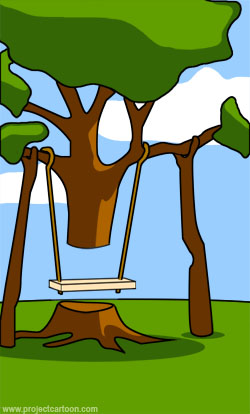
\includegraphics[width=0.9\columnwidth]{images/howdesigned}
\caption*{\tiny \centering How the analyst designed it}\label{fig:howdesigned}\end{subfigure}&
\begin{subfigure}[t]{0.15\textwidth}\centering
\includegraphics[width=0.9\columnwidth]{images/howprogrammed}
\caption*{\tiny \centering How the programmer wrote it}\label{fig:howprogrammed}\end{subfigure}&
%\begin{subfigure}{0.2\textwidth}\centering
\includegraphics[width=0.8\columnwidth]{images/howdocumented}
%\caption{How it was documented}\label{fig:howdocumented}\end{subfigure}\\
%\begin{subfigure}{0.2\textwidth}\centering
\includegraphics[width=0.85\columnwidth]{images/howinstalled}
%\caption*{\centering  What operations installed}\label{fig:howinstalled}\end{subfigure}&
%\begin{subfigure}{0.2\textwidth}\centering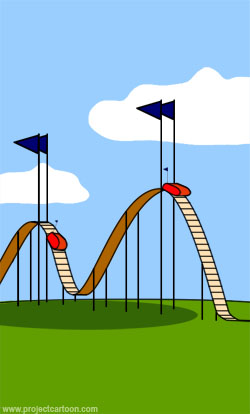
\includegraphics[width=0.8\columnwidth]{images/howbilled}
%\caption{How the customer was billed}\label{fig:howbilled}\end{subfigure}&
%\begin{subfigure}{0.2\textwidth}\centering
\includegraphics[width=0.85\columnwidth]{images/howsupported}
%\caption*{\centering How it was supported\newline}\label{fig:howsupported}\end{subfigure}&
%\begin{subfigure}[t]{0.15\textwidth}\centering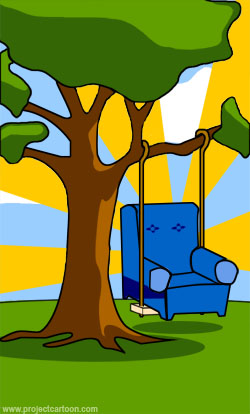
\includegraphics[width=0.9\columnwidth]{images/howdescribed}
%\caption*{\tiny \centering How it was promoted}\label{fig:howsupported}\end{subfigure}&
%\begin{subfigure}{0.2\textwidth}\centering
\includegraphics[width=0.85\columnwidth]{images/whendelivered}
%\caption*{\centering  When it was delivered\newline}\label{fig:whendelivered}\end{subfigure}\\
\begin{subfigure}[t]{0.15\textwidth}\centering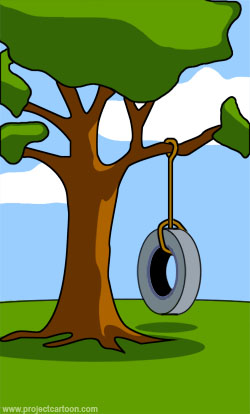
\includegraphics[width=0.9\columnwidth]{images/whatneeded}
\caption*{\tiny \centering What the user really needed}\label{fig:whatneeded}\end{subfigure}\\
\hline
\end{tabular}
\caption{Biased perception of information in the software development process, based on different mental models. [images from \cite{projectcartoon}]}
\label{fig:swingexample}
\end{center}
\end{figure}
\end{frame}

\section{Domain-Specific Modeling Languages}

\begin{frame}
\vspace{.5cm}
  \frametitle{Domain-Specific Modeling Languages}
    \begin{figure}[H]
      \centering
      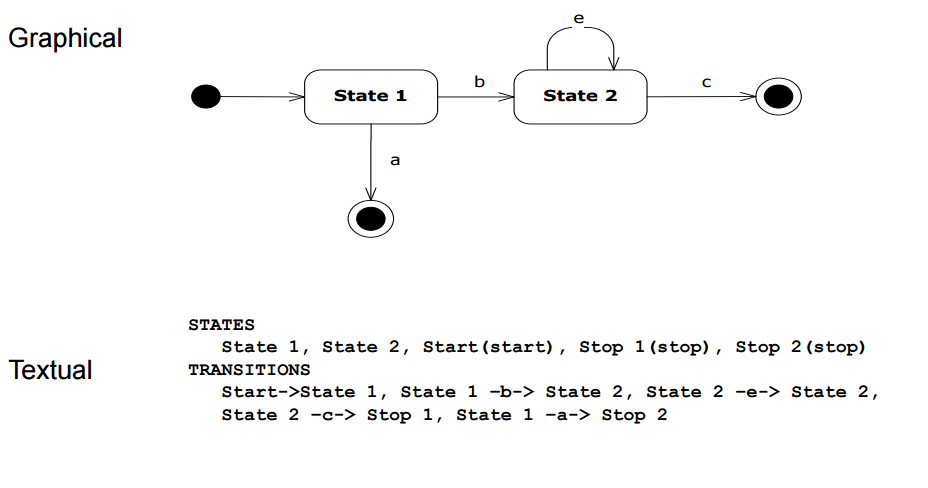
\includegraphics[width=\textwidth]{../images/GraficalTextualComparison.PNG}
      \label{compare:textgraphiclang}
    \end{figure}
\end{frame}


\begin{frame}
\vspace{.5cm}
  \frametitle{Graphical Modeling Languages}
  \framesubtitle{StarLogo TNG}
  \begin{itemize}
   \item simulation of complex systems without programming skills
   \item puzzle-piece blocks: 
	\\shapes only allow syntactically correct constructs
   \item color based on function
  \end{itemize}
  
  \begin{figure}[hbtp]
	\centering
  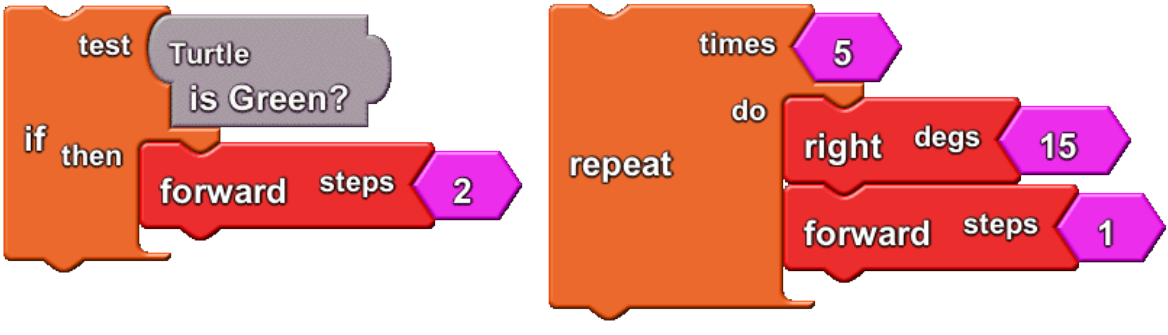
\includegraphics[width=\textwidth]{../images/StarLogoTNGBlocksEx.PNG}
	%\caption{StarLogo TNG’s graphical programming blocks.}
	\label{fig1}
  \end{figure}
\end{frame}

\begin{frame}
\vspace{-1.4cm}
  \frametitle{Graphical Modeling Languages}
  \framesubtitle{LEGO Mindstorms EV3}
    \begin{table}[h!]
    \begin{center}
      \begin{tabular}{cc}
      
      \begin{subfigure}{0.5\textwidth}\centering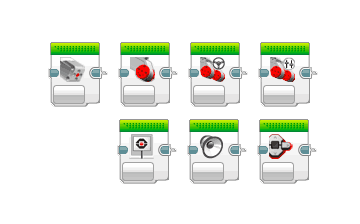
\includegraphics[width=\textwidth]{../images/LearnToProgram_action_blocks_landscape.png}\caption{action blocks}\end{subfigure}&
      \begin{subfigure}{0.5\textwidth}\centering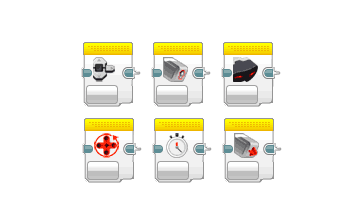
\includegraphics[width=\textwidth]{../images/LearnToProgram_sensor_blocks_landscape.png}\caption{sensor blocks}\end{subfigure}\\

      \begin{subfigure}{0.5\textwidth}\centering\caption{operation blocks}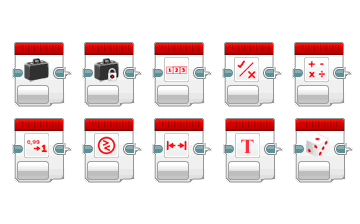
\includegraphics[width=\textwidth]{../images/LearnToProgram_operations_blocks_landscape.png}\end{subfigure}&
      \begin{subfigure}{0.5\textwidth}\centering\caption{flow blocks}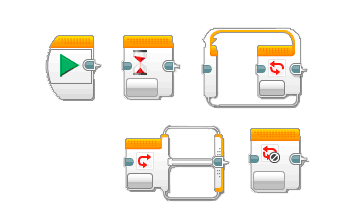
\includegraphics[width=\textwidth]{../images/LearnToProgram_flow_blocks_landscape.png}\end{subfigure}\\
      \end{tabular}
      \end{center}
    \end{table}
\end{frame}

\begin{frame}
\vspace{.5cm}
  \frametitle{Textual Modeling Languages}
  \framesubtitle{PhyDSL}
  \begin{itemize}
   \item create models for the game development domain
   \item fast prototyping of physics-based games
   \item text editor (syntax highlighting ; text completion)
  \end{itemize}

  \begin{figure}[hbtp]
      \centering
      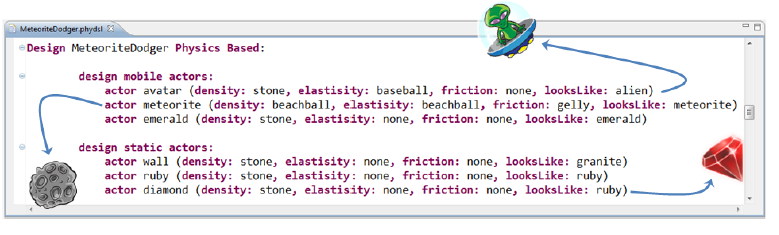
\includegraphics[width=\textwidth]{../images/PhyDSL1.PNG}
      \captionof{figure}{PhyDSL: Static Actor Definition}
    \end{figure}
\end{frame}

\section{Creating Domain-Specific Modeling Languages}
\begin{frame}
\vspace{.5cm}
  \frametitle{Creating Modeling Languages}
  \framesubtitle{Xtext}
  \begin{itemize}
    \item Grammar Rules (similar to EBNF)
    \item generates Text-Editor Plugin for Eclipse
    \item features Syntax-Highlighting; Autocompletion
  \end{itemize}
  \begin{figure}[hbtp]
      \centering
      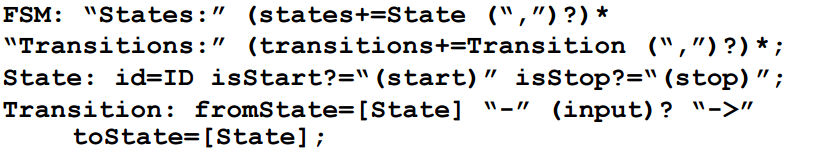
\includegraphics[width=\textwidth]{../images/XTextGrammar.PNG}
      \captionof{figure}{Xtext: Grammar for Modeling Finite State Machines}
    \end{figure}
\end{frame}

\section{Creating Domain-Specific Modeling Languages}
\begin{frame}
\vspace{.5cm}
  \frametitle{Creating Modeling Languages}
  \framesubtitle{Graphical Modeling Framework (GMF)}
  \begin{itemize}
    \item User defines Mapping: Graphical Shapes $\rightarrow$ Model-Elements
    \item GMF generates Graphical-Editor Plugin for Eclipse 
    \item features Drag \& Drop; Tooling (add/delete Elements via Menus)
  \end{itemize}
  \begin{figure}[htbp]
      \centering
      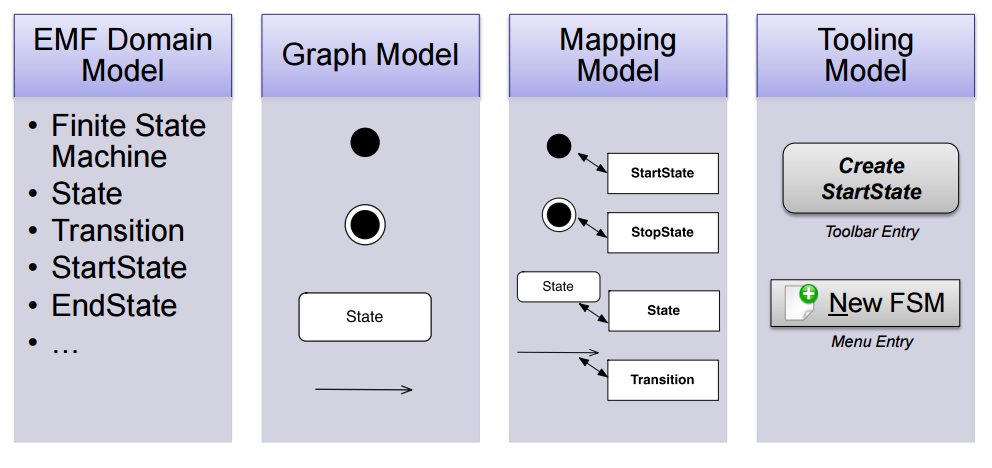
\includegraphics[width=\textwidth]{../images/TableGMFSteps.PNG}
      \captionof{figure}{Parts needed to create a graphical editor.}
      \label{mapmodel}
    \end{figure}
\end{frame}

% 4. Folie
\section{Summary}
\begin{frame}
  \vspace{2cm}
  \frametitle{Summary}
  \begin{itemize}
    \item Support Novices and Experts in Creating Models easily 
    \item Overview ofver some Modeling Languages for Novices
    \item Textual $\leftrightarrow$ Graphical Modeling Languages
    \item Example Tools for Creating Modeling Languages (Xtext \& GMF)
  \end{itemize}
\end{frame}

\appendix
\begin{frame}
\vspace{4cm}
\centering \Large \textcolor{black}{Questions?}

\end{frame}



\end{document}